\documentclass{../exam2e}

\usepackage{graphicx}

\usepackage[ngerman]{babel}


%% Seitenlayout (mit 'exam') --------
\extrawidth{1.6cm}
\extraheadheight[-1.5cm]{-1.2cm}% optionales Argument trifft auf erste Seite zu.
\extrafootheight{-1.2cm}

% oder alternativ stattdessen Seitenlayout mit 'geometry'
% \usepackage{geometry}
% \geometry{%
% 	margin=1.5cm
% }

\setlength{\parindent}{0pt}

\begin{document}
\pagestyle{empty}

% Schalter zum Drucken von Lösungen --------
% kommentieren, um Lösungen zu unterdrücken:
\printanswers
% ------------------------------------------

% Überschrift
\section*{Probeaufgaben, Mathematik 8b}

% Tabelle mit den Punkten:
\gradetable[h][questions]\\[.5ex]

% einleitender Text:
Übersichtlichkeit, Darstellung und Rechtschreibung werden bewertet.
Rechnungen müssen nach\-voll\-zieh\-bar gestaltet werden. 
Textaufgaben sollen mit einem Antwortsatz beendet werden. 
Achte bei allen Größen auf die richtige Einheit.



\subsection*{Aufgaben zum Thema Wurzeln}

\begin{questions}% Fragen --------


\begin{question}[2]
	Erkläre den Begriff der Quadratwurzel anhand des Beispiels $\sqrt{25}$.
	Nutze dazu die Fachsprache.
\end{question}

\begin{question}[4]
	Charakterisiere die folgenden Zahlen, indem du die links aufgeführten Eigenschaften jeweils in der Tabelle abhakst:
\begin{table}[htpb]
\centering
\renewcommand{\arraystretch}{1.4}
\begin{tabular}{l*{4}{p{2cm}}}
\hline
	{Die Zahl ist\ldots}	& $-4$	& $\frac{72}{12}$	& $\sqrt{11}$ 	& $\sqrt{169}$	\\
\hline
	natürlich	\\
	negativ		\\ 
\hline
	ganz		\\
	rational	\\
\hline
	irrational	\\
	reell		\\
\hline
\end{tabular}
\end{table}
\end{question}% End Aufgabe Tabelle.



\begin{question}[3]
	Berechne geschickt:
\begin{equation}
\aaa{}\quad \sqrt{2}\cdot \sqrt{18}			\qquad \qquad
\aaa{}\quad \sqrt{10}\cdot \sqrt{{3,6}}		\qquad \qquad
\aaa{}\quad \sqrt{125}\;\colon \sqrt{5}
\end{equation}
\end{question}


\subsection*{Aufgaben zum Thema Wahrscheinlichkeitsrechnung}

\begin{question}[5]
	Aus einer Tüte mit 
	3 orangenen und 2 gelben Bonbons
%	2 orangenen und 3 gelben Bonbons
	wird zweimal je ein Bonbon gezogen und nicht zurückgelegt.
\begin{subparts}
	\subpart Zeichne ein vollständiges Baumdiagramm.
\uplevel{Nutze das Baumdiagramm zur Beantwortung der folgenden Frage:}% end uplevel.
	\subpart Berechne die Wahrscheinlichkeit zwei verschiedenfarbige Bonbons zu ziehen.
\end{subparts}
\end{question}

% Lösung zur Aufgabe oben:
\begin{solution}
\begin{subparts}
	\subpart Baumdiagramm:

	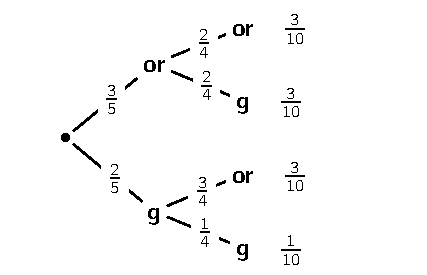
\includegraphics{baumdiagramm}

	\subpart Zu verschiedenfarbig gehören die Fälle von orange-gelb und gelb-orange. In beiden Fällen ist die Wahrscheinlichkeit gleich $\frac{3}{10}$, insgesamt also $\frac{6}{10}$.
\end{subparts}

\end{solution}


\end{questions}% Ende der Fragen --------


\clearpage
\addtocounter{page}{-1}
\thispagestyle{empty} 
\fillwithgrid{\stretch{1}}  % Kästchen

%% Eine leere Seite mit Zeilen/Kästchen zum Schreiben ---
%\clearpage
%\addtocounter{page}{-1}
%\thispagestyle{empty} 
%\fillwithgrid{\stretch{1}}  % Kästchen
%\fillwithlines{\stretch{1}} % Zeilen

%% Füge N cm leerer Zeilen/Kästchen zum Schreiben ein ---
% \fillwithgrid{Ncm}  % Kästchen, z.B. 5cm
% \fillwithlines{Ncm} % Zeilen, z.B. 5cm

%% Füge Zeilen/Kästchen bis zum Seitenende ein ---
% \fillwithgrid{\stretch{1}}  % Kästchen
% \fillwithlines{\stretch{1}} % Zeilen

\end{document}